\documentclass{beamer}
\usepackage[utf8]{inputenc}
\usepackage[squaren]{SIunits}
\usepackage{varwidth,setspace}
\usepackage{tikz}
\usetikzlibrary{intersections,positioning,backgrounds,fit,matrix,shapes,calc,decorations.pathmorphing,decorations.text}
\usetheme{default}

\newcommand*{\mimg}[2]{\begingroup
\setbox0=\hbox{\includegraphics[height=#2]{#1}}\parbox{\wd0}{\box0}\endgroup}
\newcommand*{\rmimg}[2]{\begingroup
\setbox0=\hbox{\includegraphics[angle=90,origin=c,height=#2]{#1}}\parbox{\wd0}{\box0}\endgroup}
\newcommand*{\symok}[0]{\includegraphics[height=1em]{symbol_ok.pdf}}
\newcommand*{\symbad}[0]{\includegraphics[height=1em]{symbol_bad.pdf}}
\newcommand*{\symidk}[0]{{\bf\color{blue}\Large?}}

\setbeamertemplate{navigation symbols}{}%remove navigation symbols
\setbeamertemplate{footline}{\hspace*{.5cm}\scriptsize{\hfill\raisebox{1mm}{\insertframenumber}\hspace*{.5cm}}}

\setlength{\tabcolsep}{0.5mm}

\title{Exploring the dark universe with the Atacama Cosmology Telescope}
\author{Sigurd Kirkevold Næss}
\institute{Subdepartment of astrophysics, Oxford University}
\date{October 13th, 2014}

\begin{document}

\begin{frame}
	\titlepage
	\vspace{-1cm}
	\begin{center}
	%{\footnotesize The source code of this talk can be found at {\color[rgb]{0,0.7,0}https://github.com/amaurea/talk-bmode}}
	\end{center}
\end{frame}

\begin{frame}{The physics of CMB lensing}
	\begin{center}
		\begin{tikzpicture}
			\node at (0,0) {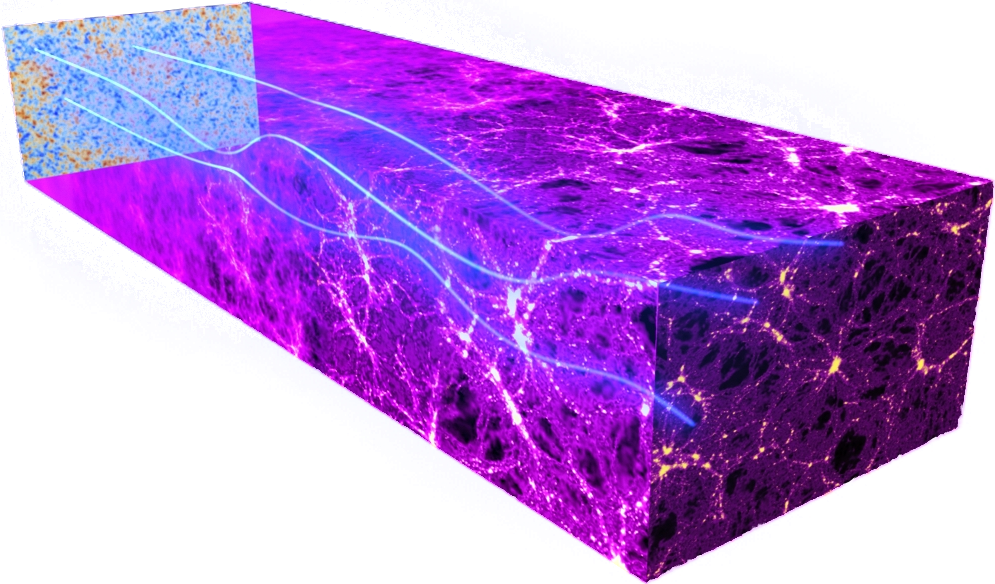
\includegraphics[width=\textwidth]{plots/Planck_gravitational_lensing_CMB_transparent.png}};
			\uncover<2->{\draw[thick,white,dashed] (-5,2.6) -- (2.4,-0.4);}
			\uncover<3->{\draw[thick,white,->] (2.4,-0.4) -- (2.8,-0.15);}
			\uncover<4->{\node[white] at (3.5,-0.5) {$\sim2$ arcmin};}
		\end{tikzpicture}

		{\footnotesize Credit: Planck, ESA}
	\end{center}
\end{frame}

\begin{frame}{Lensing distorts the CMB}
	\begin{center}
		\begin{tikzpicture}
			\only<1>{\node at (0,0) {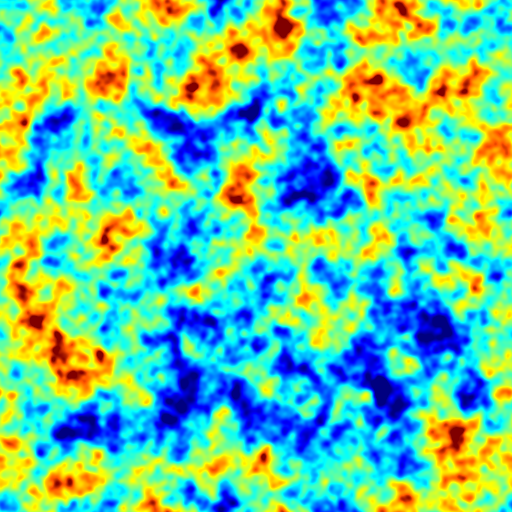
\includegraphics[height=7cm]{plots/maps/T.png}};}%
			\only<2>{\node at (0,0) {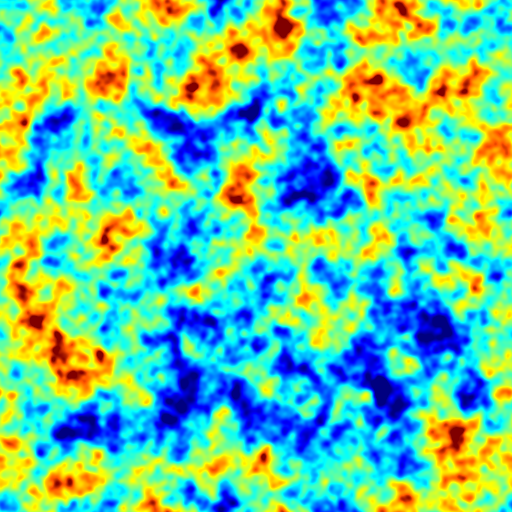
\includegraphics[height=7cm]{plots/maps/T.png}};}%
			\only<3>{\node at (0,0) {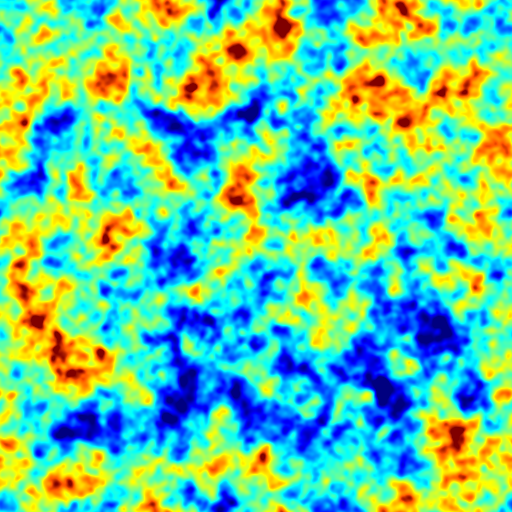
\includegraphics[height=7cm]{plots/maps/TlT.png}};}%
			\only<4-5>{\node at (0,0) {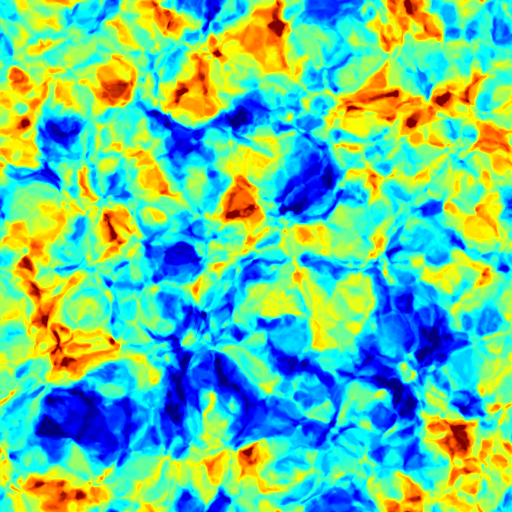
\includegraphics[height=7cm]{plots/maps/TsT.png}};}%
			\only<2-4>{\node at (0,0) {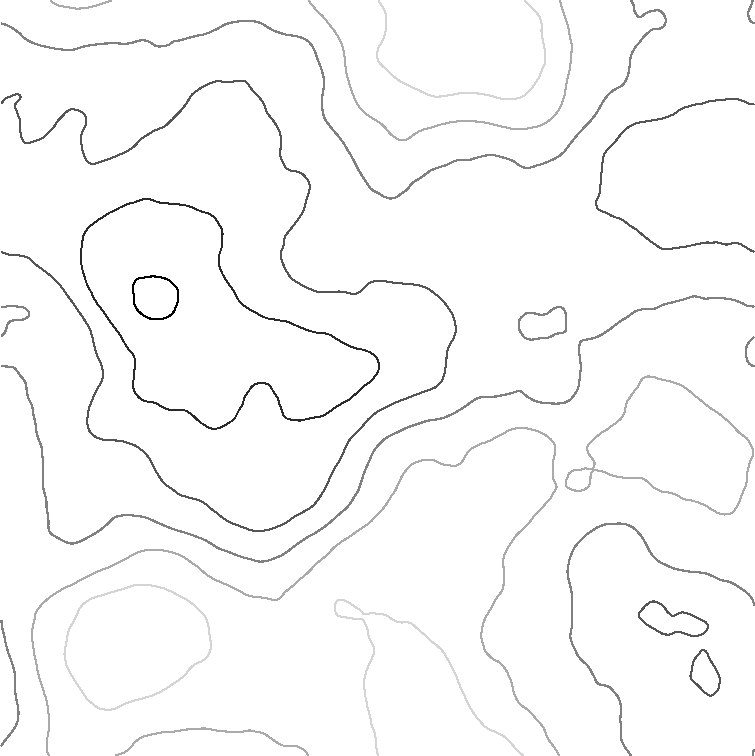
\includegraphics[height=7cm]{plots/maps/phi_contours.png}};}%
		\end{tikzpicture}

		\only<1>{Unlensed\uncover<0>{p}}%
		\only<2>{Gravitational potential}%
		\only<3>{Lensed\uncover<0>{p}}%
		\only<4>{Lensed x10\uncover<0>{p}}%
		\only<5>{Non-Gaussian\uncover<0>{p}}%
	\end{center}
\end{frame}

\begin{frame}{Lensing distorts the CMB Polarization}
	\begin{center}
		\hspace*{-3mm}
		\begin{tabular}{cc}
			{\bf Q} ($\pm 20\mu$K) & {\bf U} ($\pm 20\mu$K) \\
			\only<1>{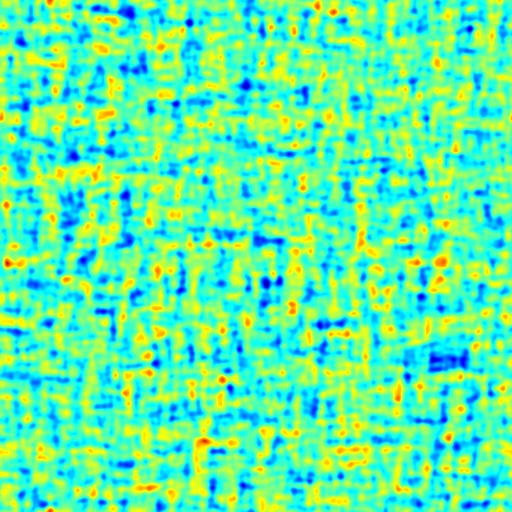
\includegraphics[height=5.5cm]{plots/maps/EBQ.png}}%
			\only<2>{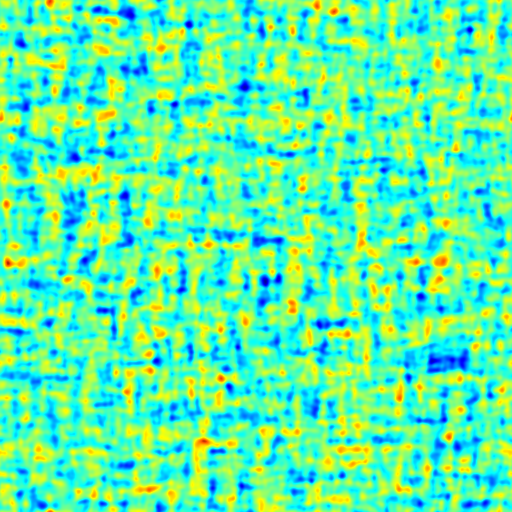
\includegraphics[height=5.5cm]{plots/maps/EBlQ.png}}%
			&
			\only<1>{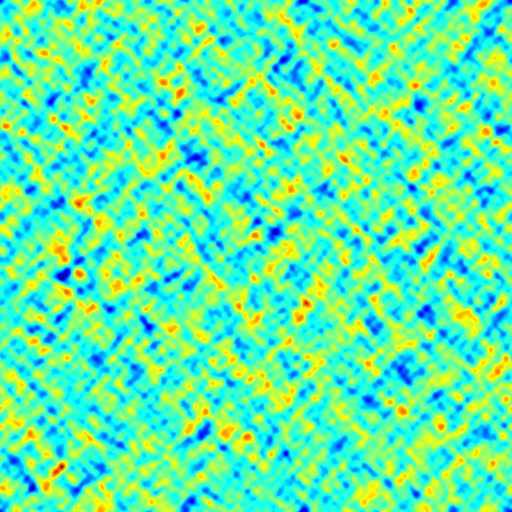
\includegraphics[height=5.5cm]{plots/maps/EBU.png}}%
			\only<2>{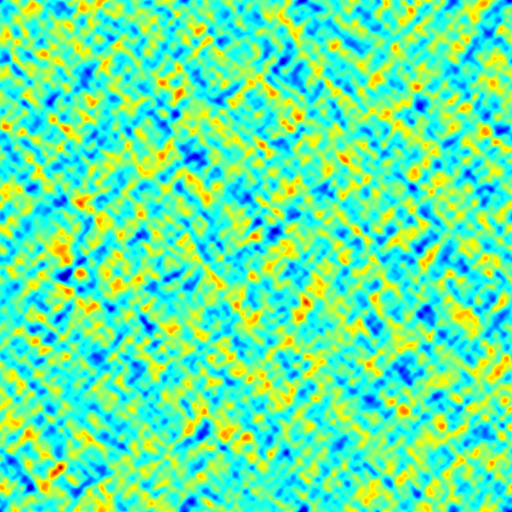
\includegraphics[height=5.5cm]{plots/maps/EBlU.png}}%
		\end{tabular}

		\only<1>{Unlensed}%
		\only<2>{Lensed}%
	\end{center}
\end{frame}

\begin{frame}{E, B and Q, U}
	\begin{center}
		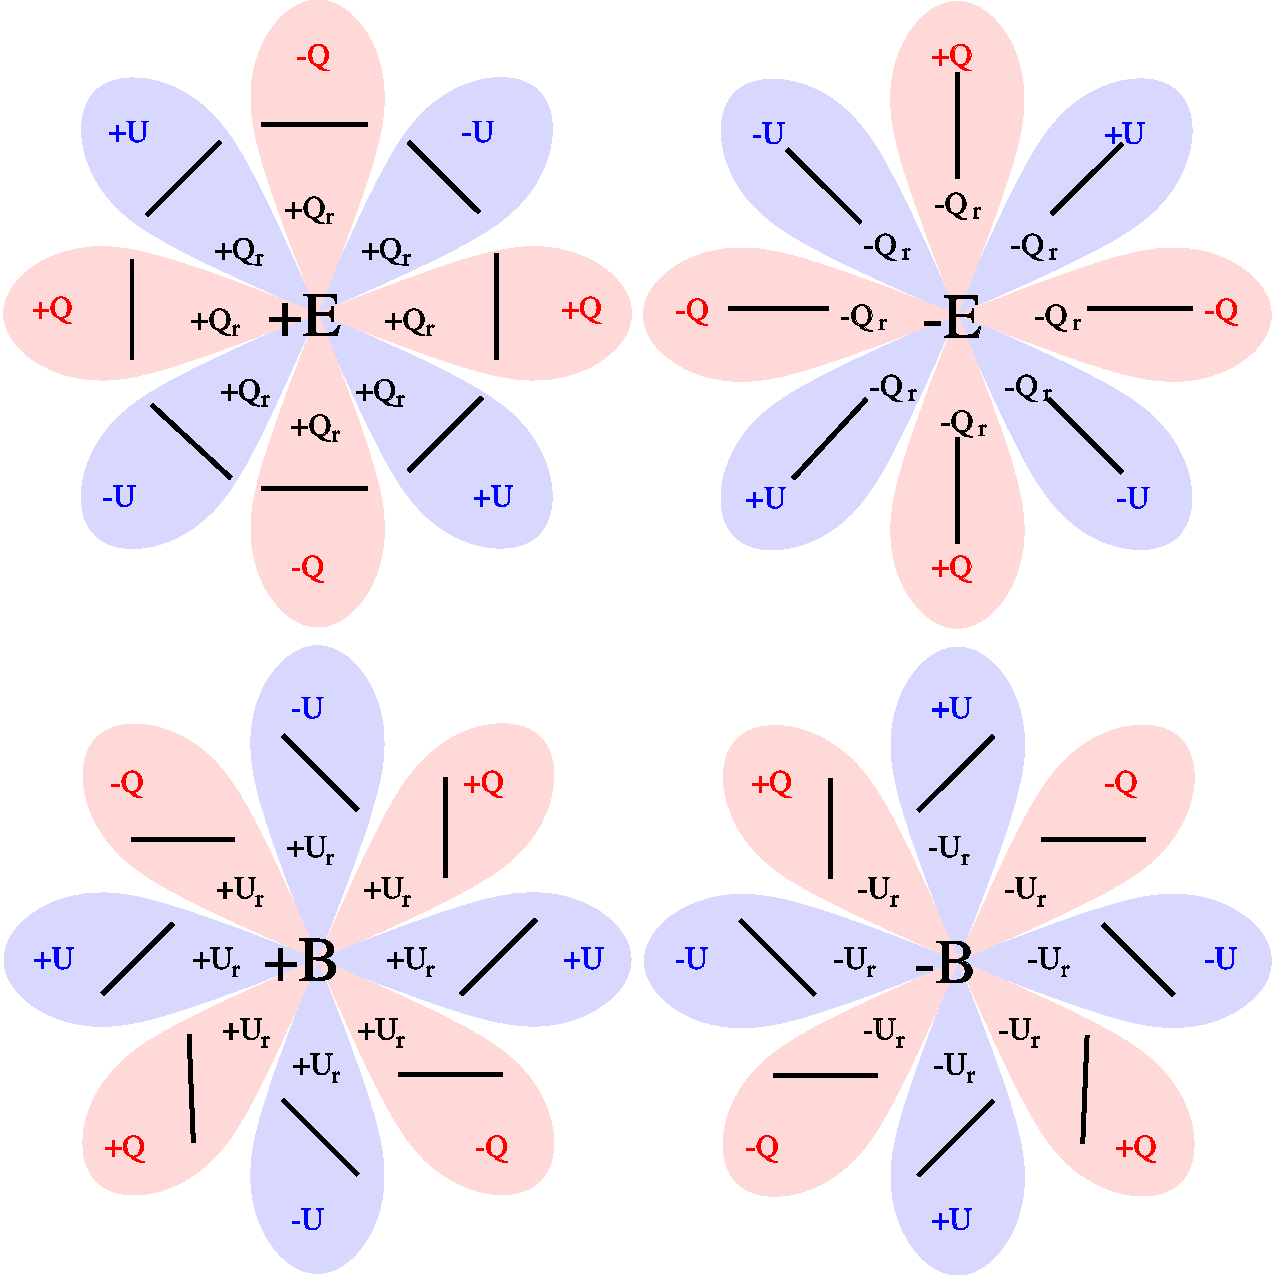
\includegraphics[height=8cm]{plots/EB_healpix.pdf}
	\end{center}
\end{frame}

\begin{frame}{E,B and Q, U}
	\begin{center}
		\only<1>{E and B result from quadrupole-convolutions of Q and U}%
		\only<2>{Reverse also holds}%

	\scalebox{1.7}{
		\begin{minipage}{5cm}
			\begin{align*}
				\only<1>{%
				E =& \rmimg{plots/queb_0.png}{1cm} \otimes Q + \mimg{plots/queb_2.png}{1cm} \otimes U \\
				B =& \mimg{plots/queb_1.png}{1cm} \otimes Q + \rmimg{plots/queb_3.png}{1cm} \otimes U}%
				\only<2>{%
				Q =& \rmimg{plots/ebqu_0.png}{1cm} \otimes E + \mimg{plots/ebqu_2.png}{1cm} \otimes B \\
				U =& \mimg{plots/ebqu_1.png}{1cm} \otimes E + \rmimg{plots/ebqu_3.png}{1cm} \otimes B}%
			\end{align*}
		\end{minipage}}
	\end{center}
\end{frame}

\begin{frame}{Lensing distorts E and B}
	\begin{center}
		\hspace*{-3mm}
		\begin{tabular}{cc}
			{\bf E} ($\pm 20\mu$K) & {\bf B} ($\pm 0.5\mu$K) \\
			\only<1>{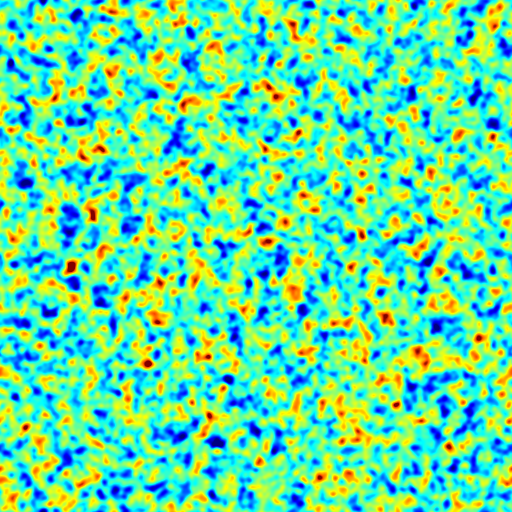
\includegraphics[height=5.5cm]{plots/maps/E.png}}%
			\only<2>{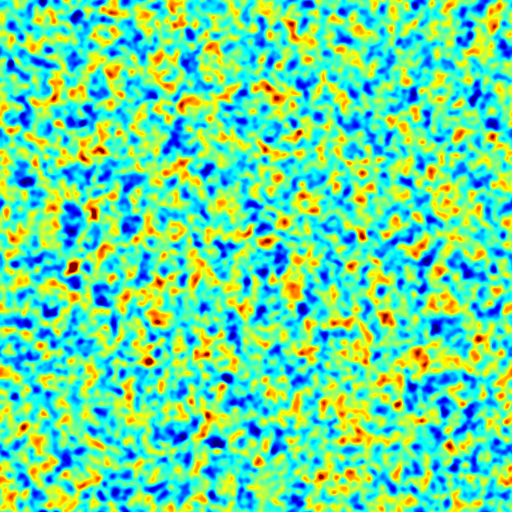
\includegraphics[height=5.5cm]{plots/maps/EBlE.png}}%
			&
			\only<1>{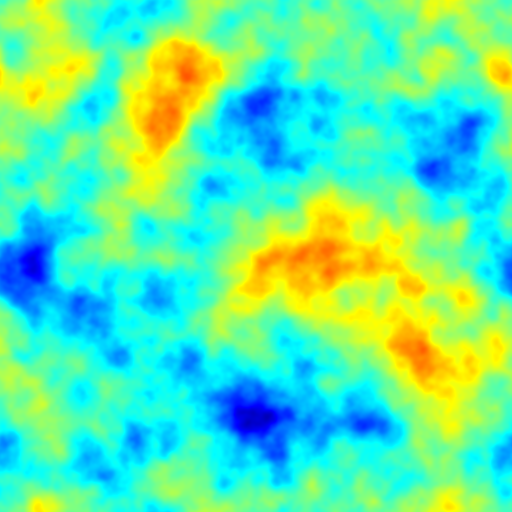
\includegraphics[height=5.5cm]{plots/maps/B.png}}%
			\only<2>{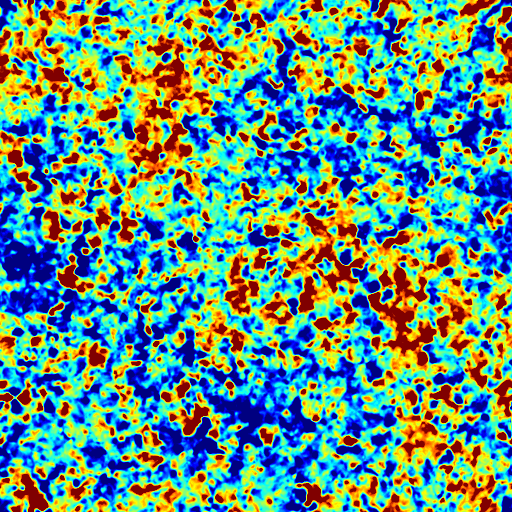
\includegraphics[height=5.5cm]{plots/maps/EBlB.png}}%
		\end{tabular}

		\only<1>{Unlensed}%
		\only<2>{Lensed}%
	\end{center}
\end{frame}

\begin{frame}{Lensing distorts the power spectra}
	\begin{center}
		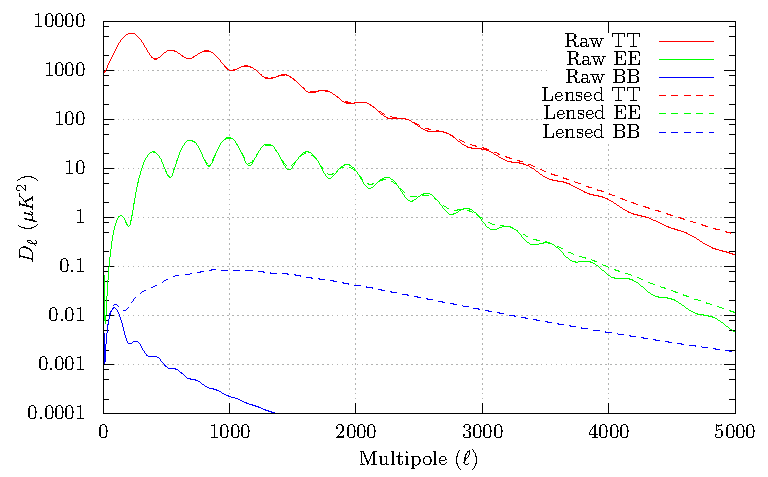
\includegraphics[width=\textwidth]{plots/spectra.pdf}
	\end{center}
\end{frame}

\begin{frame}{Disentangling CMB and lensing}
	\begin{center}
		\begin{itemize}
			\item Lensing correlates previously uncorrelated multipoles
				\begin{tabular}{lll}
					Before & $\langle T(\mathbf{l}_1)T(\mathbf{l}_2)\rangle = 0$ & for $\mathbf{l}_1 \ne \mathbf{l}_2$ \\
					After &  $\langle T(\mathbf{l}_1)T(\mathbf{l}_2)\rangle \propto \phi(\mathbf{l}_1+\mathbf{l}_2)$ & for $\mathbf{l}_1 \ne \mathbf{l}_2$
				\end{tabular}
			\item \uncover<2->{Use cross-correlations to reconstruct lensing potential}
				\begin{tikzpicture}
					\node at (0,0) {%
						$\begin{aligned}
							\uncover<3->{%
							\begin{matrix}
								\textrm{\tiny lensed T}\left\{\mimg{plots/maps/TlT.png}{2cm}\right. \\
								\textrm{\tiny lensed E}\left\{\mimg{plots/maps/EBlE.png}{2cm}\right. \\
								\textrm{\tiny lensed B}\left\{\mimg{plots/maps/EBlB.png}{2cm}\right.
							\end{matrix}}
							\uncover<4->{%
							\rightarrow
							\underbrace{\mimg{plots/maps/phi.png}{2cm}}_{\textrm{\tiny lensing potential }\phi}}
							\uncover<5->{%
							\rightarrow
							\begin{matrix}
								\left.\mimg{plots/maps/T.png}{2cm}\right\}\textrm{\tiny true T} \\
								\left.\mimg{plots/maps/E.png}{2cm}\right\}\textrm{\tiny true E} \\
								\left.\mimg{plots/maps/B.png}{2cm}\right\}\textrm{\tiny true B}
							\end{matrix}}
					\end{aligned}$};
					\uncover<6->{\draw[thick,red] (0.15,-0.25) circle (1.62);}
			\end{tikzpicture}
		\end{itemize}
	\end{center}
\end{frame}

\begin{frame}{Pure CMB is degenerate}
	\begin{center}
		\vspace{-10mm}
		\begin{tikzpicture}
			\node at ( 4.15,0.12) {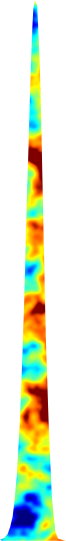
\includegraphics[height=4.2cm]{plots/cmb_slice.png}};
			\node at ( 0.00,0.00) {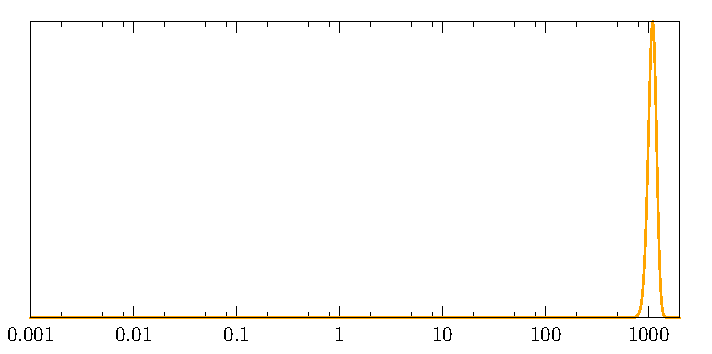
\includegraphics[width=10cm]{plots/z_cmb.pdf}};
			\node[orange] at (4.15,2.40) {CMB};
			\node at (-5.20,0.20) {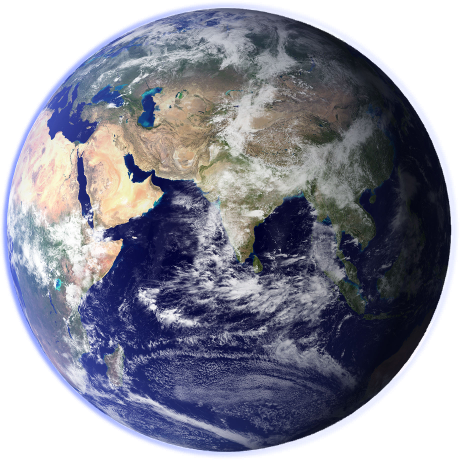
\includegraphics[height=1.0cm]{plots/earth.png}};
			\uncover<14->{%
			\node at ( 0.00,0.00) {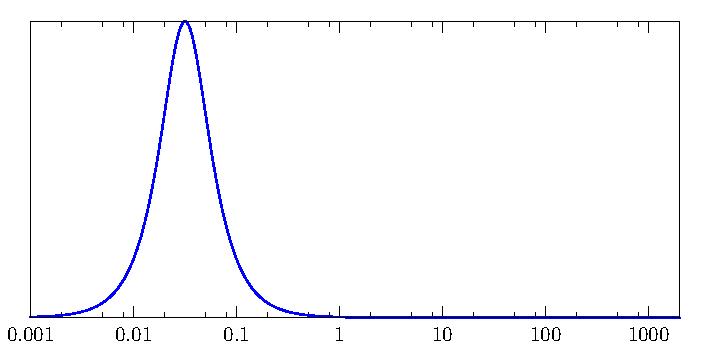
\includegraphics[width=10cm]{plots/z_sn.pdf}};
			\node[blue] at (-2.40,2.40) {SN};}
			\uncover<15->{%
			\node at ( 0.00,0.00) {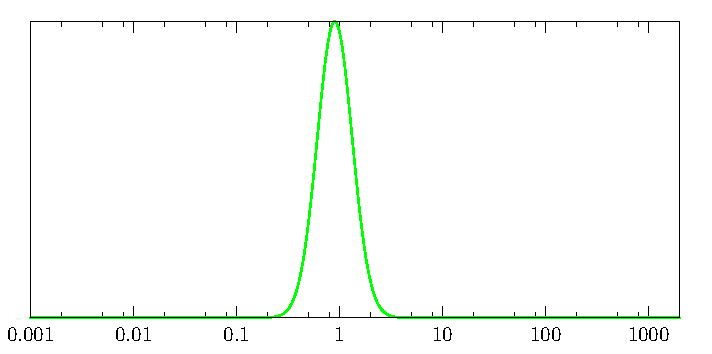
\includegraphics[width=10cm]{plots/z_bao.pdf}};
			\node[green] at (-0.32,2.40) {BAO};}
			\uncover<18->{%
			\node at ( 0.00,0.00) {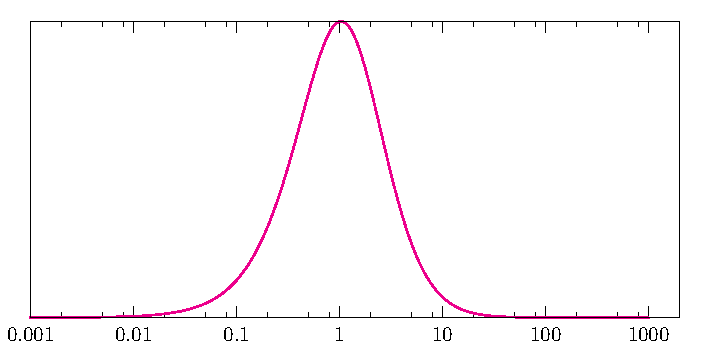
\includegraphics[width=10cm]{plots/z_lens.pdf}};
			\node[magenta,align=center] at (-0.24,0.00) {CMB\\Lensing};}

			\uncover<2-11>{%
			\draw[thick,red] (4.15,0.26) ellipse (0.4 and 2.5);}
			\uncover<3-11>{%
			\draw[ultra thick,red,<->] (-4.2,2.4) -- (3.6,2.4);
			\node[red] at (0.0,2.7) {$d_A$};}
			\uncover<4-11>{%
			\node[blue,scale=2] at (0,0.2) {\Huge ?};}

			\node at (0,-4) {$\begin{aligned}
				\uncover<5->{\mimg{plots/maps/degen1.png}{2cm}}
				\uncover<6->{\xrightarrow{-\Omega_\Lambda}}
				\uncover<7->{\mimg{plots/maps/degen2.png}{2cm}}
				\uncover<8->{\xrightarrow{+t_0}}
				\uncover<9->{\mimg{plots/maps/degen3.png}{2cm}}
				\uncover<10->{\xrightarrow{+\Omega_k}}
				\uncover<11->{\mimg{plots/maps/degen1.png}{2cm}}
				\end{aligned}$};

			\uncover<12>{\node[fill=white,align=center] at (0,-1.5) {
				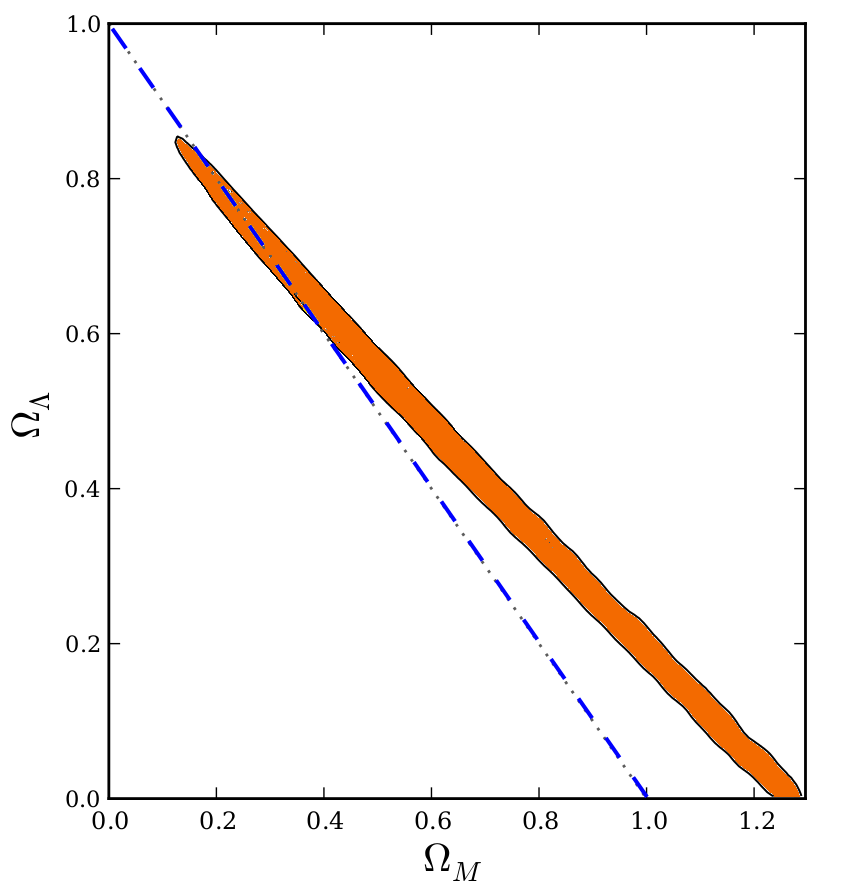
\includegraphics[height=7.5cm]{plots/cmb_nolens_degen.png}\\
				{\footnotesize Modified from Sherwin et al. 2011 \uncover<0>{g}}};}
			\uncover<16>{\node[fill=white,align=center] at (0,-1.5) {
				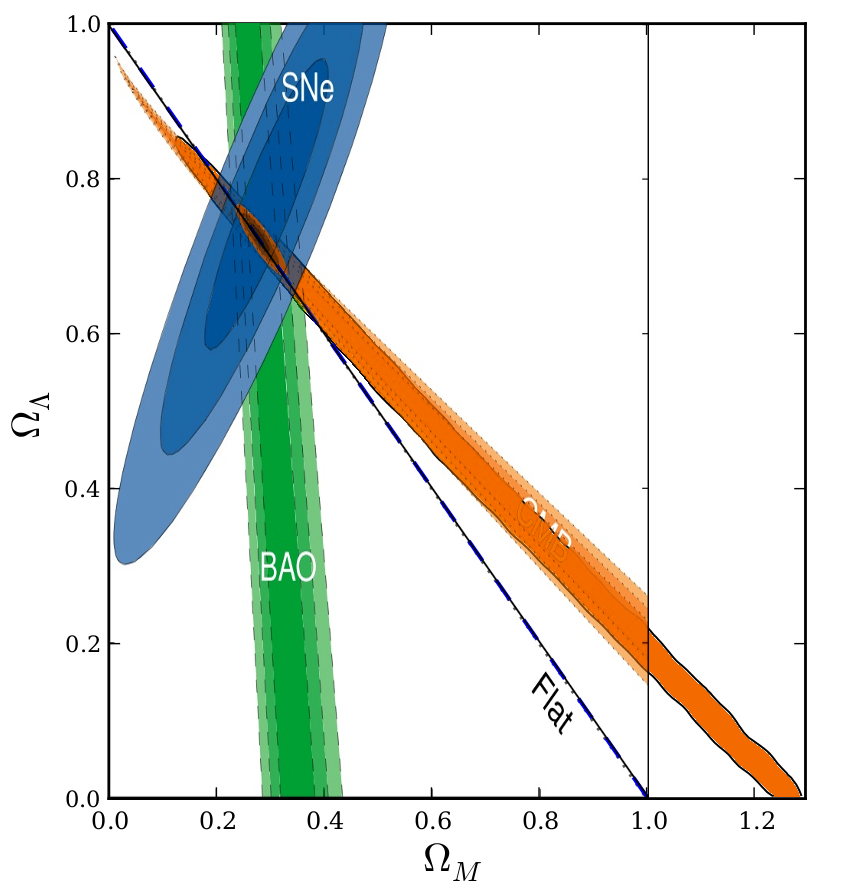
\includegraphics[height=7.5cm]{plots/cmb_nolens_sn_bao.png}\\
				{\footnotesize Modified from Supernova Cosmology Project 2010}};}

		\end{tikzpicture}
	\end{center}
\end{frame}

\begin{frame}{Good systematics}
	\begin{itemize}
		\item Linear physics (mostly)

	\end{itemize}
\end{frame}

\begin{frame}{Observational status}
\end{frame}

\begin{frame}{(Near) future}
\end{frame}

\end{document}
